% !TEX root = ../../presentation.tex

\begin{slide}{Op Layer}
  \pause
  
\includegraphics[scale=0.4]{stickman}

  \textbf{Bob}
\end{slide}

\begin{slide}{im2col}
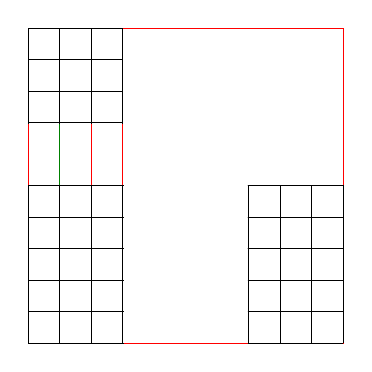
\begin{tikzpicture}
  % R layer (feature map)
  \yzplane{0}{
    \draw [NavyBlue] (0, 0) rectangle ++(4, 4);
  }
  \xyplane{4}{
    \draw [NavyBlue] (0, 0) rectangle ++(0.4, 4);
  }
  \xzplane{0}{
    \draw [NavyBlue] (0, 0) rectangle ++(0.4, 4);
  }
  \xzplane{4}{
    \draw [NavyBlue] (0, 0) rectangle ++(0.4, 4);
  }

  % G layer (feature map)
  \yzplane{0.4}{
    \draw [Green] (0, 0) rectangle ++(4, 4);
  }
  \xyplane{0}{
    \draw [Green] (0.4, 0) rectangle ++(0.4, 4);
  }
  \xyplane{4}{
    \draw [Green] (0.4, 0) rectangle ++(0.4, 4);
  }
  \xzplane{0}{
    \draw [Green] (0.4, 0) rectangle ++(0.4, 4);
  }
  \xzplane{4}{
    \draw [Green] (0.4, 0) rectangle ++(0.4, 4);
  }

  % B layer (feature map)
  \yzplane{0.8}{
    \draw [Red] (0, 0) rectangle ++(4, 4);
  }
  \xyplane{0}{
    \draw [Red] (0.8, 0) rectangle ++(0.4, 4);
  }
  \xyplane{4}{
    \draw [Red] (0.8, 0) rectangle ++(0.4, 4);
  }
  \xzplane{0}{
    \draw [Red] (0.8, 0) rectangle ++(0.4, 4);
  }
  \xzplane{4}{
    \draw [Red] (0.8, 0) rectangle ++(0.4, 4);
  }

  \foreach \i/\j in {0/1, 0/2, 0.4/3, 0.8/4, 0.8/5, 0.8/6, 0.8/7, 0.8/8, 0.8/9}
  {
  \only<\j>{
    \xyplane{\i}{
      \draw (0, 2.79) grid [step=0.4] ++(1.2, 1.21);
    }
    \xyplane{{\i+1.2}}{
      \draw (0, 2.79) grid [step=0.4] ++(1.2, 1.21);
    }
    \yzplane{0}{
      \draw (2.79, \i) grid [step=0.4] ++(1.21, 1.21);
    }
    \yzplane{1.2}{
      \draw (2.79, \i) grid [step=0.4] ++(1.21, 1.21);
    }
    \xzplane{4}{
      \draw (0, \i) grid [step=0.4] ++(1.21, 1.21);
    }
    \xzplane{2.8}{
      \draw (0, \i) grid [step=0.4] ++(1.21, 1.21);
    }
  }
  }
\end{tikzpicture}
\hspace{1cm}
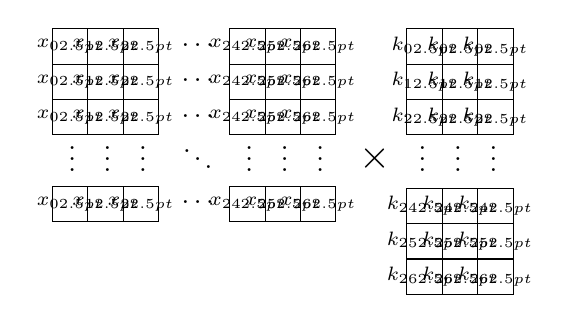
\begin{tikzpicture}
  \foreach \i in {2, ..., 4} {
    \onslide<\i->{
      \foreach \x in {0, ..., 2} {
        \draw ({\x * 0.45}, {(4 - \i) * 0.45}) rectangle ++(0.45, 0.45)
              node [midway] {\scriptsize$x_{\scaleto{\x}{2.5pt}}$};
      }
      \draw (1.845, {(4 - \i) * 0.45 + 0.245}) node {$\dots$};
      \foreach \x in {24, ..., 26} {
        \draw ({(\x - 19) * 0.45}, {(4 - \i) * 0.45}) rectangle ++(0.45, 0.45)
              node [midway] {\scriptsize$x_{\scaleto{\x}{2.5pt}}$};
      }
    }
  }

  \onslide<5->{
    \foreach \i in {1, 2, 3, 6, 7, 8} {
        \draw ({\i * 0.45 - 0.2}, -0.2) node {$\vdots$};
    }
    \foreach \x in {0, ..., 2} {
      \draw ({\x * 0.45}, -1.1) rectangle ++(0.45, 0.45)
            node [midway] {\scriptsize$x_{\scaleto{\x}{2.5pt}}$};
    }
    \draw (1.845, -0.2) node {$\ddots$};
    \draw (1.845, -0.855) node {$\dots$};
    \foreach \x in {24, ..., 26} {
      \draw ({(\x - 19) * 0.45}, -1.1) rectangle ++(0.45, 0.45)
            node [midway] {\scriptsize$x_{\scaleto{\x}{2.5pt}}$};
    }
  }

  \onslide<9> { \draw (4.1, -0.3) node {\Large$\times$};}

  \foreach \i in {6, 7, 8} {
    \onslide<\i-> {
      \foreach \y in {0, ..., 2} {
        \draw ({4.5 + (\i - 6) * 0.45}, {(2 - \y) * 0.45})
              rectangle ++(0.45, 0.45)
              node [midway] {\scriptsize$k_{\scaleto{\y}{2.5pt}}$};
      }
      \draw ({4.7 + (\i - 6) * 0.45}, -0.2) node {$\vdots$};
      \foreach \y in {24, ..., 26} {
        \draw ({4.5 + (\i - 6) * 0.45}, {(21.5 - \y) * 0.45})
              rectangle ++(0.45, 0.45)
              node [midway] {\scriptsize$k_{\scaleto{\y}{2.5pt}}$};
      }
    }
  }
\end{tikzpicture}
\vspace{1cm}
\end{slide}
